% Options for packages loaded elsewhere
\PassOptionsToPackage{unicode}{hyperref}
\PassOptionsToPackage{hyphens}{url}
\PassOptionsToPackage{dvipsnames,svgnames,x11names}{xcolor}
%
\documentclass[
  us-letterpaper,
]{scrreprt}

\usepackage{amsmath,amssymb}
\usepackage{iftex}
\ifPDFTeX
  \usepackage[T1]{fontenc}
  \usepackage[utf8]{inputenc}
  \usepackage{textcomp} % provide euro and other symbols
\else % if luatex or xetex
  \usepackage{unicode-math}
  \defaultfontfeatures{Scale=MatchLowercase}
  \defaultfontfeatures[\rmfamily]{Ligatures=TeX,Scale=1}
\fi
\usepackage{lmodern}
\ifPDFTeX\else  
    % xetex/luatex font selection
\fi
% Use upquote if available, for straight quotes in verbatim environments
\IfFileExists{upquote.sty}{\usepackage{upquote}}{}
\IfFileExists{microtype.sty}{% use microtype if available
  \usepackage[]{microtype}
  \UseMicrotypeSet[protrusion]{basicmath} % disable protrusion for tt fonts
}{}
\makeatletter
\@ifundefined{KOMAClassName}{% if non-KOMA class
  \IfFileExists{parskip.sty}{%
    \usepackage{parskip}
  }{% else
    \setlength{\parindent}{0pt}
    \setlength{\parskip}{6pt plus 2pt minus 1pt}}
}{% if KOMA class
  \KOMAoptions{parskip=half}}
\makeatother
\usepackage{xcolor}
\setlength{\emergencystretch}{3em} % prevent overfull lines
\setcounter{secnumdepth}{5}
% Make \paragraph and \subparagraph free-standing
\ifx\paragraph\undefined\else
  \let\oldparagraph\paragraph
  \renewcommand{\paragraph}[1]{\oldparagraph{#1}\mbox{}}
\fi
\ifx\subparagraph\undefined\else
  \let\oldsubparagraph\subparagraph
  \renewcommand{\subparagraph}[1]{\oldsubparagraph{#1}\mbox{}}
\fi

\usepackage{color}
\usepackage{fancyvrb}
\newcommand{\VerbBar}{|}
\newcommand{\VERB}{\Verb[commandchars=\\\{\}]}
\DefineVerbatimEnvironment{Highlighting}{Verbatim}{commandchars=\\\{\}}
% Add ',fontsize=\small' for more characters per line
\usepackage{framed}
\definecolor{shadecolor}{RGB}{241,243,245}
\newenvironment{Shaded}{\begin{snugshade}}{\end{snugshade}}
\newcommand{\AlertTok}[1]{\textcolor[rgb]{0.68,0.00,0.00}{#1}}
\newcommand{\AnnotationTok}[1]{\textcolor[rgb]{0.37,0.37,0.37}{#1}}
\newcommand{\AttributeTok}[1]{\textcolor[rgb]{0.40,0.45,0.13}{#1}}
\newcommand{\BaseNTok}[1]{\textcolor[rgb]{0.68,0.00,0.00}{#1}}
\newcommand{\BuiltInTok}[1]{\textcolor[rgb]{0.00,0.23,0.31}{#1}}
\newcommand{\CharTok}[1]{\textcolor[rgb]{0.13,0.47,0.30}{#1}}
\newcommand{\CommentTok}[1]{\textcolor[rgb]{0.37,0.37,0.37}{#1}}
\newcommand{\CommentVarTok}[1]{\textcolor[rgb]{0.37,0.37,0.37}{\textit{#1}}}
\newcommand{\ConstantTok}[1]{\textcolor[rgb]{0.56,0.35,0.01}{#1}}
\newcommand{\ControlFlowTok}[1]{\textcolor[rgb]{0.00,0.23,0.31}{#1}}
\newcommand{\DataTypeTok}[1]{\textcolor[rgb]{0.68,0.00,0.00}{#1}}
\newcommand{\DecValTok}[1]{\textcolor[rgb]{0.68,0.00,0.00}{#1}}
\newcommand{\DocumentationTok}[1]{\textcolor[rgb]{0.37,0.37,0.37}{\textit{#1}}}
\newcommand{\ErrorTok}[1]{\textcolor[rgb]{0.68,0.00,0.00}{#1}}
\newcommand{\ExtensionTok}[1]{\textcolor[rgb]{0.00,0.23,0.31}{#1}}
\newcommand{\FloatTok}[1]{\textcolor[rgb]{0.68,0.00,0.00}{#1}}
\newcommand{\FunctionTok}[1]{\textcolor[rgb]{0.28,0.35,0.67}{#1}}
\newcommand{\ImportTok}[1]{\textcolor[rgb]{0.00,0.46,0.62}{#1}}
\newcommand{\InformationTok}[1]{\textcolor[rgb]{0.37,0.37,0.37}{#1}}
\newcommand{\KeywordTok}[1]{\textcolor[rgb]{0.00,0.23,0.31}{#1}}
\newcommand{\NormalTok}[1]{\textcolor[rgb]{0.00,0.23,0.31}{#1}}
\newcommand{\OperatorTok}[1]{\textcolor[rgb]{0.37,0.37,0.37}{#1}}
\newcommand{\OtherTok}[1]{\textcolor[rgb]{0.00,0.23,0.31}{#1}}
\newcommand{\PreprocessorTok}[1]{\textcolor[rgb]{0.68,0.00,0.00}{#1}}
\newcommand{\RegionMarkerTok}[1]{\textcolor[rgb]{0.00,0.23,0.31}{#1}}
\newcommand{\SpecialCharTok}[1]{\textcolor[rgb]{0.37,0.37,0.37}{#1}}
\newcommand{\SpecialStringTok}[1]{\textcolor[rgb]{0.13,0.47,0.30}{#1}}
\newcommand{\StringTok}[1]{\textcolor[rgb]{0.13,0.47,0.30}{#1}}
\newcommand{\VariableTok}[1]{\textcolor[rgb]{0.07,0.07,0.07}{#1}}
\newcommand{\VerbatimStringTok}[1]{\textcolor[rgb]{0.13,0.47,0.30}{#1}}
\newcommand{\WarningTok}[1]{\textcolor[rgb]{0.37,0.37,0.37}{\textit{#1}}}

\providecommand{\tightlist}{%
  \setlength{\itemsep}{0pt}\setlength{\parskip}{0pt}}\usepackage{longtable,booktabs,array}
\usepackage{calc} % for calculating minipage widths
% Correct order of tables after \paragraph or \subparagraph
\usepackage{etoolbox}
\makeatletter
\patchcmd\longtable{\par}{\if@noskipsec\mbox{}\fi\par}{}{}
\makeatother
% Allow footnotes in longtable head/foot
\IfFileExists{footnotehyper.sty}{\usepackage{footnotehyper}}{\usepackage{footnote}}
\makesavenoteenv{longtable}
\usepackage{graphicx}
\makeatletter
\def\maxwidth{\ifdim\Gin@nat@width>\linewidth\linewidth\else\Gin@nat@width\fi}
\def\maxheight{\ifdim\Gin@nat@height>\textheight\textheight\else\Gin@nat@height\fi}
\makeatother
% Scale images if necessary, so that they will not overflow the page
% margins by default, and it is still possible to overwrite the defaults
% using explicit options in \includegraphics[width, height, ...]{}
\setkeys{Gin}{width=\maxwidth,height=\maxheight,keepaspectratio}
% Set default figure placement to htbp
\makeatletter
\def\fps@figure{htbp}
\makeatother

\usepackage{upgreek}
\usepackage{amsmath}
\usepackage{amssymb}
\usepackage{tikz}
\newcommand{\dashedbox}[1]{
  \begin{tikzpicture}
    \node[draw, dashed, rounded corners=5pt, inner sep=10pt] {
      \begin{minipage}{0.8\textwidth} % Establece el ancho del minipage
        #1
      \end{minipage}
    };
  \end{tikzpicture}
}
\makeatletter
\makeatother
\makeatletter
\@ifpackageloaded{bookmark}{}{\usepackage{bookmark}}
\makeatother
\makeatletter
\@ifpackageloaded{caption}{}{\usepackage{caption}}
\AtBeginDocument{%
\ifdefined\contentsname
  \renewcommand*\contentsname{Tabla de contenidos}
\else
  \newcommand\contentsname{Tabla de contenidos}
\fi
\ifdefined\listfigurename
  \renewcommand*\listfigurename{Listado de Figuras}
\else
  \newcommand\listfigurename{Listado de Figuras}
\fi
\ifdefined\listtablename
  \renewcommand*\listtablename{Listado de Tablas}
\else
  \newcommand\listtablename{Listado de Tablas}
\fi
\ifdefined\figurename
  \renewcommand*\figurename{Figura}
\else
  \newcommand\figurename{Figura}
\fi
\ifdefined\tablename
  \renewcommand*\tablename{Tabla}
\else
  \newcommand\tablename{Tabla}
\fi
}
\@ifpackageloaded{float}{}{\usepackage{float}}
\floatstyle{ruled}
\@ifundefined{c@chapter}{\newfloat{codelisting}{h}{lop}}{\newfloat{codelisting}{h}{lop}[chapter]}
\floatname{codelisting}{Listado}
\newcommand*\listoflistings{\listof{codelisting}{Listado de Listados}}
\usepackage{amsthm}
\theoremstyle{definition}
\newtheorem{definition}{Definición}[chapter]
\theoremstyle{plain}
\newtheorem{theorem}{Teorema}[chapter]
\theoremstyle{remark}
\AtBeginDocument{\renewcommand*{\proofname}{Prueba}}
\newtheorem*{remark}{Observación}
\newtheorem*{solution}{Solución}
\makeatother
\makeatletter
\@ifpackageloaded{caption}{}{\usepackage{caption}}
\@ifpackageloaded{subcaption}{}{\usepackage{subcaption}}
\makeatother
\makeatletter
\@ifpackageloaded{tcolorbox}{}{\usepackage[skins,breakable]{tcolorbox}}
\makeatother
\makeatletter
\@ifundefined{shadecolor}{\definecolor{shadecolor}{rgb}{.97, .97, .97}}
\makeatother
\makeatletter
\makeatother
\makeatletter
\makeatother
\ifLuaTeX
\usepackage[bidi=basic]{babel}
\else
\usepackage[bidi=default]{babel}
\fi
\babelprovide[main,import]{spanish}
% get rid of language-specific shorthands (see #6817):
\let\LanguageShortHands\languageshorthands
\def\languageshorthands#1{}
\ifLuaTeX
  \usepackage{selnolig}  % disable illegal ligatures
\fi
\IfFileExists{bookmark.sty}{\usepackage{bookmark}}{\usepackage{hyperref}}
\IfFileExists{xurl.sty}{\usepackage{xurl}}{} % add URL line breaks if available
\urlstyle{same} % disable monospaced font for URLs
\hypersetup{
  pdftitle={Ecuación de Langevin y su aplicación en la predicción de terremotos},
  pdfauthor={Pavel Santiago Hernandez Hernandez; Asesor Yofre Hernán García Gómez},
  pdflang={es},
  colorlinks=true,
  linkcolor={blue},
  filecolor={Maroon},
  citecolor={Blue},
  urlcolor={Blue},
  pdfcreator={LaTeX via pandoc}}

\title{Ecuación de Langevin y su aplicación en la predicción de
terremotos}
\author{Pavel Santiago Hernandez Hernandez \and Asesor Yofre Hernán
García Gómez}
\date{2027-01-06}

\begin{document}
\begin{titlepage}
\hspace{-1.7cm} %Este comando es para mandar a la izquierda ;)
%Aquí empiezan los tres minipages de antes
\begin{minipage}[t][0.03\textheight][c]{0.22\textwidth}
        
\includegraphics[width=3.0cm]{assets/UNACH.png}
\end{minipage}\hspace{0.9cm}
\begin{minipage}[t][0.03\textheight][c]{0.69\textwidth}
\begin{center}
                \textsc{\huge Universidad Autónoma de Chiapas}\\[0.3cm]
                \hrule height 2.5pt
                \vspace{0.2cm}
                \hrule height1pt
                \vspace{0.3cm}
                \textsc{\Large Facultad de Ciencias en Física y Matemáticas}
\end{center}
\end{minipage}\hspace{0.2cm}
\begin{minipage}[t][0.03\textheight][c]{0.2\textwidth}
		
\includegraphics[width=2.7cm]{assets/logofcfm.png}
\end{minipage}\\
%%%%%%%%%%%%%%%%%%Aquí comienzan los otros dos minipages del título%%%%%%%%%%%%%%%%%%%%%%%%%%%%%%%%%%%%%%%%%%%%%%%%%%%%%%%%%%%%%%%%%%%%%%%%%%%%%%%%%%%%%%%%%%%%%%
\begin{minipage}[t][0.93\textheight][c]{0.06\textwidth}
\vspace{60pt}
    \begin{center}
        \vrule width1pt height18cm
        \vspace{5mm}
        \vrule width2.5pt height18cm
        \vspace{5mm}
        \vrule width1pt height18cm
   \end{center}
\end{minipage}\hspace{1.3cm} %Esto mueve las letras que tienes ahí
\begin{minipage}[t][0.95\textheight][c]{0.76\textwidth}

            \begin{center}
                {\Large\bfseries Ecuación de Langevane y su aplicación en la predicción de terremotos}\\[2cm]
                \textsc{\huge \textbf{T\, E\, S\, I\, S}}\\[1.5cm]
                \textsc{\large QUE PARA OBTENER EL TÍTULO DE:}\\[0.3cm]
                \textbf{\textsc{LICENCIADO EN MATEMÁTICAS}}\\[1.5cm]
                \textsc{\large PRESENTA:}\\[0.3cm]
                \textbf{\textsc{\large {PAVEL SANTIAGO HERNANDEZ HERNANDEZ}}}\\[2cm]
                {\large\scshape Director:\\[0.3cm]
                {\textbf{\large Dr. Yofre Hernán García Gómez }}}\\[2.0cm]
                \large{Tuxtla Gutiérrez, Chiapas a - de - del 2024.}

            \end{center}
\end{minipage}
\end{titlepage}

%\pagebreak[2]

%\chapter*{Dedicatoria}
%\begin{flushright}
%\textit{A mis padres, \\ por su inquebrantable fe en mí y por ser mi inspiración para perseguir la excelencia. Esta tesis es mi manera de agradecerles su amor, paciencia y sacrificio.}
%\end{flushright}


\ifdefined\Shaded\renewenvironment{Shaded}{\begin{tcolorbox}[boxrule=0pt, borderline west={3pt}{0pt}{shadecolor}, enhanced, interior hidden, breakable, frame hidden, sharp corners]}{\end{tcolorbox}}\fi

\renewcommand*\contentsname{Tabla de contenidos}
{
\hypersetup{linkcolor=}
\setcounter{tocdepth}{2}
\tableofcontents
}
\bookmarksetup{startatroot}

\hypertarget{resumen}{%
\chapter*{Resumen}\label{resumen}}
\addcontentsline{toc}{chapter}{Resumen}

\markboth{Resumen}{Resumen}

Esta tesis presenta

\bookmarksetup{startatroot}

\hypertarget{introducciuxf3n}{%
\chapter{Introducción}\label{introducciuxf3n}}

\hypertarget{introducciuxf3n-del-modelo-de-langevin-y-su-aplicaciuxf3n-a-terremotos}{%
\section{Introducción del modelo de Langevin y su aplicación a
terremotos}\label{introducciuxf3n-del-modelo-de-langevin-y-su-aplicaciuxf3n-a-terremotos}}

El modelo de Langevin fue propuesto por Paul Langevin en 1908 para
describir el movimiento browniano de partículas suspendidas en un
fluido. Este modelo captura la dinámica de una partícula bajo la
influencia de una fuerza determinista (como la fricción) y una fuerza
aleatoria (ruido blanco gaussiano), y se expresa mediante una ecuación
diferencial estocástica de la forma:

\begin{equation}\protect\hypertarget{eq-Langevin}{}{ 
dv(t) = -\gamma v(t)\,dt + \sqrt{2D}\,dW(t) 
}\label{eq-Langevin}\end{equation}

donde de Ecuación~\ref{eq-Langevin}:

\begin{itemize}
\tightlist
\item
  \(v(t)\): velocidad de la partícula,
\item
  \(\gamma\): coeficiente de fricción,
\item
  \(D\): coeficiente de difusión (intensidad del ruido térmico),
\item
  \(W(t)\): movimiento browniano estándar.
\end{itemize}

Con el tiempo, este modelo fue generalizado para describir sistemas que
combinan comportamientos deterministas con fluctuaciones aleatorias,
incluyendo fenómenos físicos, biológicos, químicos y financieros.

En el contexto geofísico, el modelo de Langevin se ha extendido para
modelar la dinámica de fallas sísmicas. Para representar eventos
sísmicos abruptos ---como rupturas en la corteza terrestre--- se
incorpora un término adicional de saltos, modelados mediante un proceso
de Poisson o, más generalmente, un proceso de Lévy. El modelo extendido
es:

\[
dv(t) = [-\gamma v(t) + F_{\text{ext}}(t)]\,dt + \sqrt{2D}\,dW(t) + dJ(t),
\]

donde:

\begin{itemize}
\tightlist
\item
  \(( F_{\text{ext}}(t) )\): fuerza externa acumulada, por ejemplo, por
  tectónica de placas,
\item
  \(( J(t) )\): proceso de saltos, que representa eventos súbitos
  (rupturas sísmicas),
\item
  El resto de símbolos mantienen su significado anterior.
\end{itemize}

Una formulación típica para los saltos es:

\[
J(t) = \sum_{i=1}^{N(t)} Y_i,
\]

donde:

\begin{itemize}
\tightlist
\item
  \(( N(t) )\) es un proceso de Poisson de tasa \((\lambda> 0 )\),
\item
  \(( Y_i )\) representa la magnitud del i-ésimo salto (aleatoria, por
  ejemplo, con distribución exponencial o normal truncada).
\end{itemize}

Este modelo se denomina Ecuación de Langevin con saltos y pertenece a la
clase de ecuaciones diferenciales estocásticas impulsadas por procesos
de Lévy.

Su aplicación en geofísica permite modelar:

\begin{itemize}
\tightlist
\item
  El movimiento gradual de una falla mediante la fricción y ruido
  térmico,
\item
  La ocurrencia de microtemblores,
\item
  La irrupción de terremotos mayores como saltos discontinuos.
\end{itemize}

Este enfoque ofrece una base matemática para la simulación y el análisis
estadístico de secuencias sísmicas, incluyendo la estimación de
probabilidades de ocurrencia, clasificación de eventos y simulación de
trayectorias dinámicas realistas.

\bookmarksetup{startatroot}

\hypertarget{objetivos}{%
\chapter{Objetivos}\label{objetivos}}

\hypertarget{los-objetivos-de-este-proyecto-se-estaruxe1n-afinando-dentro-de-las-proximas-semanas.}{%
\section{Los objetivos de este proyecto se estarán afinando dentro de
las proximas
semanas.}\label{los-objetivos-de-este-proyecto-se-estaruxe1n-afinando-dentro-de-las-proximas-semanas.}}

\bookmarksetup{startatroot}

\hypertarget{presentaciuxf3n-sonora}{%
\chapter{Presentación sonora}\label{presentaciuxf3n-sonora}}

\hypertarget{introducciuxf3n-1}{%
\section{Introducción}\label{introducciuxf3n-1}}

El análisis de la recurrencia sísmica representa un pilar fundamental
dentro de la sismología estadística. Un enfoque riguroso para abordar
esta problemática consiste en modelar la ocurrencia y evolución de los
sismos mediante un proceso estocástico de tiempo discreto,
específicamente utilizando cadenas de Markov.

Este marco metodológico permite representar los estados de intensidad
sísmica ---definidos mediante intervalos de magnitud como baja, media y
alta--- y examinar las probabilidades de transición entre ellos. A
partir de series temporales de registros sísmicos, se construye una
estructura probabilística que caracteriza el comportamiento recurrente
de los sismos y provee estimaciones cuantitativas del riesgo sísmico
futuro.

El artículo `'Estimates of earthquake recurrences in the Chiayi--Tainan
area, Taiwan'', publicado en 2002, aborda un tema de gran relevancia
para la sismología y la gestión de riesgos naturales: la estimación de
la recurrencia de terremotos en una región altamente sísmica del
suroeste de Taiwán.

Los temas abordados en dicho articulo son los siguientes:

\begin{enumerate}
\def\labelenumi{\roman{enumi}.}
\item
  Ley de Gutenburg - Richter.
\item
  Cadenas de Markov.
\item
  Tiene como objetivo estudiar los periodos de retorno para los
  terremotos de distinta escala.
\item
  Se calcula a partir de la amplitud de las ondas sísmicas registradas
  en un sismografo.
\end{enumerate}

\hypertarget{escala-richter}{%
\subsection{Escala Richter}\label{escala-richter}}

\begin{enumerate}
\def\labelenumi{\roman{enumi}.}
\item
  Es una escala logarítmica que cuantifica la energía liberada por un
  terremoto, basada en la amplitud máxima de las ondas sísmicas
  registradas.
\item
  La magnitud se calcula mediante la fórmula: \[
  M = \log_{10}(A) - \log_{10}(A_0)
  \] donde \(A\) es la amplitud medida y \(A_0\) es un valor de
  referencia dependiente de la distancia al epicentro.
\item
  Permite comparar la intensidad de diferentes eventos sísmicos y
  clasificar su peligrosidad.
\end{enumerate}

\hypertarget{definiciones}{%
\section{Definiciones}\label{definiciones}}

\begin{definition}[Espacio de Estados y Clasificación de INtensidades de
sísmos]\protect\hypertarget{def-varmues}{}\label{def-varmues}

Sea \(M:=\{M_1,M_2,\ldots, M_k\}\) el conjunto finito de estados de
intensidad sísmica, definimos como intervalos en la escala de Richter de
la siguiente manera:

\begin{enumerate}
\def\labelenumi{\roman{enumi}.}
\item
  \(M_2\): Sismos de encala entre \(2\leq M_2\leq 2.9\)
\item
  \(M_3\): Sismos de encala entre \(3\leq M_3\leq 3.9\)
\item
  \(M_4\): Sismos de encala entre \(4\leq M_4\leq 4.9\)
\item
  \(M_5\): Sismos de encala entre \(5\leq M_5\leq 5.9\)
\item
  \(M_6\): Sismos de encala entre \(6\leq M_6\leq 6.9\)
\item
  \(M_7\): Sismos de encala entre \(7\leq M_7\leq 7.9\).
\end{enumerate}

Cada sismo captado se clasifica en un estado \(M_i\) correspondiente a
su magnitud, generando una serie temporal categórica
\(\{X_t\}_{t=0}^{T}\), donde \(X_t\in M\)

\end{definition}

\begin{definition}[Proceso
estocástico]\protect\hypertarget{def-varmues}{}\label{def-varmues}

Un proceso estocástico es un modelo matemático que describe la evolución
probabilística de un sistema a lo largo del tiempo o el espacio. Se
define formalmente como una familia de variables aleatorias, donde cada
una representa el estado del sistema en un momento o posición
específicos.

Esta familia se denota como: \[\{X_t\}_{t\in T}.\] Donde:

\begin{enumerate}
\def\labelenumi{\roman{enumi}.}
\item
  \(X_t\) es la variable aleatoria que representa el estado del sistema
  en el instante \(t\).
\item
  \(T\) es el conjunto de índices (por ejemplo, un intervalo de tiempo o
  una región espacial).
\end{enumerate}

\end{definition}

\begin{definition}[Proceso de
Markov]\protect\hypertarget{def-varmues}{}\label{def-varmues}

Es un proceso estocástico \(\{X_n\}_{n\in T}\), que cumple: \[
\begin{aligned}
P(X_{n+1}=x_{n+1}|& X_n=x_n,\ X_{n-1}=x_{n-1},\ldots,X_0=x_0)\\ 
& =P(X_{n+1}=x_{n+1}|X_n=x_n)
\end{aligned}
\]

\end{definition}

\begin{definition}[Matriz de
transición]\protect\hypertarget{def-varmues}{}\label{def-varmues}

A partir de la serie de datos sísmicos clasificados, es posible
construir la matriz de transición \[
P:[p_{ij}], \ p_{ij}=P(X_{t+1}=M_j|X_t=M_i)
\] Con la propiedad de que cada fila de \(P\) es una distribución de
probabilidad, vale decir \[
\sum\limits_{j=1}^{k} p_{ij}=1,\ p_{ij}\geq 0\ \ \forall i,j
\]

\end{definition}

\bookmarksetup{startatroot}

\hypertarget{formulaciuxf3n}{%
\chapter{Formulación}\label{formulaciuxf3n}}

\begin{enumerate}
\def\labelenumi{\roman{enumi}.}
\item
  Analiza la periodicidad de terremotos en la región de Chiayi-Tainan,
  Taiwán, utilizando Cadenas de Markov.
\item
  Revelan un patrón significativo en la recurrencia de terremotos.
\item
  Demuestran que las cadenas de Markov son una herramienta efectiva para
  modelar el comportamiento sísmico.
\item
  Son útiles para la evaluación del riesgo sísmico en la región.
\end{enumerate}

Se categorizarón los siguientes cinturones sísmicos:

\begin{enumerate}
\def\labelenumi{\roman{enumi}.}
\item
  Zona sísmica occidental (WSZ).
\item
  Zona sísmica oriental (ESZ).
\item
  Zona sísmica noroeste (NSZ).
\end{enumerate}

La zona de estudio cuenta con doce fallas activas. Los terremotos se
cuantifican con la escla de magnitud local de Richter, representada como
\(M_L\), donde \(L\) representa la magnitud, \((M)\), del sísmo, por
ejemplo, la categoría \(M_4\) representa sísmos de magitud entre \(4\) y
\(4.9\). En este estudio se prepararon dos bases de datos:

\begin{enumerate}
\def\labelenumi{\roman{enumi}.}
\item
  \(M_L\geq 4\) con \(283\) eventos de 1990 a 1995.
\item
  \(M_L\geq 2\) con \(3816\) eventos de 1973 a 1995.
\end{enumerate}

\bookmarksetup{startatroot}

\hypertarget{anuxe1lisis-con-matrices-de-transiciuxf3n}{%
\chapter{Análisis con matrices de
transición}\label{anuxe1lisis-con-matrices-de-transiciuxf3n}}

Si la ocurrencia de un terremoto está estrechamente relacionada con la
replica anterior, se puede aplicar un análisis de cadenas de Markov
especificada con una transición de un paso para estudiar la periodicidad
sísmica y obtener las aproximaciones de las probabilidades de
transición.

\bookmarksetup{startatroot}

\hypertarget{simulaciuxf3n-de-trayectorias-y-eventos-suxedsmicos}{%
\chapter{Simulación de trayectorias y eventos
sísmicos}\label{simulaciuxf3n-de-trayectorias-y-eventos-suxedsmicos}}

El siguiente código genera trayectorias con ruido y eventos cuando se
supera un umbral crítico de velocidad.

\begin{Shaded}
\begin{Highlighting}[]
\ImportTok{import}\NormalTok{ numpy }\ImportTok{as}\NormalTok{ np}
\ImportTok{import}\NormalTok{ pandas }\ImportTok{as}\NormalTok{ pd}
\ImportTok{import}\NormalTok{ matplotlib.pyplot }\ImportTok{as}\NormalTok{ plt}

\CommentTok{\# {-}{-}{-} Parámetros base {-}{-}{-}}
\NormalTok{gamma }\OperatorTok{=} \FloatTok{0.8}
\NormalTok{Fext }\OperatorTok{=} \FloatTok{1.0}
\NormalTok{D }\OperatorTok{=} \FloatTok{0.5}
\NormalTok{lambda\_poisson }\OperatorTok{=} \FloatTok{1.0}   \CommentTok{\# tasa de saltos por segundo}
\NormalTok{jump\_mean }\OperatorTok{=} \FloatTok{1.0}        \CommentTok{\# media del tamaño del salto (exponencial)}
\NormalTok{jump\_scale }\OperatorTok{=} \FloatTok{0.5}       \CommentTok{\# desviación típica o escala del salto}
\NormalTok{dt }\OperatorTok{=} \FloatTok{0.01}
\NormalTok{T }\OperatorTok{=} \FloatTok{10.0}
\NormalTok{N }\OperatorTok{=} \BuiltInTok{int}\NormalTok{(T }\OperatorTok{/}\NormalTok{ dt)}
\NormalTok{n\_traj }\OperatorTok{=} \DecValTok{10}

\NormalTok{t }\OperatorTok{=}\NormalTok{ np.linspace(}\DecValTok{0}\NormalTok{, T, N)}
\NormalTok{v }\OperatorTok{=}\NormalTok{ np.zeros((n\_traj, N))}

\CommentTok{\# {-}{-}{-} Simulación con saltos de Poisson {-}{-}{-}}
\ControlFlowTok{for}\NormalTok{ i }\KeywordTok{in} \BuiltInTok{range}\NormalTok{(n\_traj):}
    \ControlFlowTok{for}\NormalTok{ n }\KeywordTok{in} \BuiltInTok{range}\NormalTok{(N }\OperatorTok{{-}} \DecValTok{1}\NormalTok{):}
\NormalTok{        dW }\OperatorTok{=}\NormalTok{ np.sqrt(dt) }\OperatorTok{*}\NormalTok{ np.random.randn()}
\NormalTok{        dN }\OperatorTok{=}\NormalTok{ np.random.poisson(lambda\_poisson }\OperatorTok{*}\NormalTok{ dt)}
\NormalTok{        jump }\OperatorTok{=}\NormalTok{ np.}\BuiltInTok{sum}\NormalTok{(np.random.normal(loc}\OperatorTok{=}\NormalTok{jump\_mean, scale}\OperatorTok{=}\NormalTok{jump\_scale, size}\OperatorTok{=}\NormalTok{dN)) }\ControlFlowTok{if}\NormalTok{ dN }\OperatorTok{\textgreater{}} \DecValTok{0} \ControlFlowTok{else} \FloatTok{0.0}
\NormalTok{        v[i, n }\OperatorTok{+} \DecValTok{1}\NormalTok{] }\OperatorTok{=}\NormalTok{ v[i, n] }\OperatorTok{+}\NormalTok{ (}\OperatorTok{{-}}\NormalTok{gamma }\OperatorTok{*}\NormalTok{ v[i, n] }\OperatorTok{+}\NormalTok{ Fext) }\OperatorTok{*}\NormalTok{ dt }\OperatorTok{+}\NormalTok{ np.sqrt(}\DecValTok{2} \OperatorTok{*}\NormalTok{ D) }\OperatorTok{*}\NormalTok{ dW }\OperatorTok{+}\NormalTok{ jump}

\CommentTok{\# {-}{-}{-} Gráfica de trayectorias {-}{-}{-}}
\NormalTok{plt.figure(figsize}\OperatorTok{=}\NormalTok{(}\DecValTok{12}\NormalTok{, }\DecValTok{6}\NormalTok{))}
\ControlFlowTok{for}\NormalTok{ i }\KeywordTok{in} \BuiltInTok{range}\NormalTok{(n\_traj):}
\NormalTok{    plt.plot(t, v[i], label}\OperatorTok{=}\SpecialStringTok{f"Trayectoria }\SpecialCharTok{\{}\NormalTok{i}\OperatorTok{+}\DecValTok{1}\SpecialCharTok{\}}\SpecialStringTok{"}\NormalTok{)}
\NormalTok{plt.xlabel(}\StringTok{"Tiempo"}\NormalTok{)}
\NormalTok{plt.ylabel(}\StringTok{"Velocidad $v(t)$"}\NormalTok{)}
\NormalTok{plt.title(}\StringTok{"10 trayectorias del modelo Langevin con saltos de Poisson"}\NormalTok{)}
\NormalTok{plt.grid(}\VariableTok{True}\NormalTok{)}
\NormalTok{plt.tight\_layout()}
\NormalTok{plt.show()}
\CommentTok{\# {-}{-}{-} Eventos sísmicos basados en umbral {-}{-}{-}}
\NormalTok{threshold }\OperatorTok{=} \FloatTok{1.0}
\NormalTok{all\_mags }\OperatorTok{=}\NormalTok{ []}

\ControlFlowTok{for}\NormalTok{ i }\KeywordTok{in} \BuiltInTok{range}\NormalTok{(n\_traj):}
\NormalTok{    mags }\OperatorTok{=}\NormalTok{ v[i, v[i] }\OperatorTok{\textgreater{}}\NormalTok{ threshold]   }\CommentTok{\# eventos donde velocidad supera umbral}
\NormalTok{    mags }\OperatorTok{=} \FloatTok{1.0} \OperatorTok{+}\NormalTok{ (mags }\OperatorTok{{-}}\NormalTok{ threshold) }\OperatorTok{*} \FloatTok{1.5}   \CommentTok{\# transformación a magnitud sísmica}
\NormalTok{    all\_mags.extend(mags)}

\CommentTok{\# Clasificación de magnitudes}
\KeywordTok{def}\NormalTok{ classify\_event(mag):}
    \ControlFlowTok{if}\NormalTok{ mag }\OperatorTok{\textless{}} \FloatTok{2.0}\NormalTok{:}
        \ControlFlowTok{return} \StringTok{\textquotesingle{}Micro\textquotesingle{}}
    \ControlFlowTok{elif} \FloatTok{2.0} \OperatorTok{\textless{}=}\NormalTok{ mag }\OperatorTok{\textless{}} \FloatTok{4.0}\NormalTok{:}
        \ControlFlowTok{return} \StringTok{\textquotesingle{}Minor\textquotesingle{}}
    \ControlFlowTok{elif} \FloatTok{4.0} \OperatorTok{\textless{}=}\NormalTok{ mag }\OperatorTok{\textless{}} \FloatTok{6.0}\NormalTok{:}
        \ControlFlowTok{return} \StringTok{\textquotesingle{}Moderate\textquotesingle{}}
    \ControlFlowTok{else}\NormalTok{:}
        \ControlFlowTok{return} \StringTok{\textquotesingle{}Strong\textquotesingle{}}

\NormalTok{event\_classes }\OperatorTok{=}\NormalTok{ [classify\_event(m) }\ControlFlowTok{for}\NormalTok{ m }\KeywordTok{in}\NormalTok{ all\_mags]}

\CommentTok{\# DataFrame de eventos}
\NormalTok{df\_events }\OperatorTok{=}\NormalTok{ pd.DataFrame(\{}\StringTok{\textquotesingle{}Magnitude\textquotesingle{}}\NormalTok{: all\_mags, }\StringTok{\textquotesingle{}Class\textquotesingle{}}\NormalTok{: event\_classes\})}
\NormalTok{states }\OperatorTok{=}\NormalTok{ [}\StringTok{\textquotesingle{}Micro\textquotesingle{}}\NormalTok{, }\StringTok{\textquotesingle{}Minor\textquotesingle{}}\NormalTok{, }\StringTok{\textquotesingle{}Moderate\textquotesingle{}}\NormalTok{, }\StringTok{\textquotesingle{}Strong\textquotesingle{}}\NormalTok{]}

\CommentTok{\# {-}{-}{-} Matriz de conteo de transiciones {-}{-}{-}}
\NormalTok{transition\_counts }\OperatorTok{=}\NormalTok{ pd.DataFrame(}\DecValTok{0}\NormalTok{, index}\OperatorTok{=}\NormalTok{states, columns}\OperatorTok{=}\NormalTok{states)}
\ControlFlowTok{for}\NormalTok{ i }\KeywordTok{in} \BuiltInTok{range}\NormalTok{(}\BuiltInTok{len}\NormalTok{(event\_classes) }\OperatorTok{{-}} \DecValTok{1}\NormalTok{):}
\NormalTok{    from\_state }\OperatorTok{=}\NormalTok{ event\_classes[i]}
\NormalTok{    to\_state }\OperatorTok{=}\NormalTok{ event\_classes[i }\OperatorTok{+} \DecValTok{1}\NormalTok{]}
\NormalTok{    transition\_counts.loc[from\_state, to\_state] }\OperatorTok{+=} \DecValTok{1}

\CommentTok{\# {-}{-}{-} Matriz de transición {-}{-}{-}}
\NormalTok{transition\_matrix }\OperatorTok{=}\NormalTok{ transition\_counts.div(transition\_counts.}\BuiltInTok{sum}\NormalTok{(axis}\OperatorTok{=}\DecValTok{1}\NormalTok{), axis}\OperatorTok{=}\DecValTok{0}\NormalTok{)}

\BuiltInTok{print}\NormalTok{(}\StringTok{"Matriz de transición de Markov basada en trayectorias simuladas:"}\NormalTok{)}
\BuiltInTok{print}\NormalTok{(transition\_matrix.}\BuiltInTok{round}\NormalTok{(}\DecValTok{3}\NormalTok{))}
\CommentTok{\# {-}{-}{-} Visualización de la matriz de transición {-}{-}{-}}
\NormalTok{plt.figure(figsize}\OperatorTok{=}\NormalTok{(}\DecValTok{6}\NormalTok{, }\DecValTok{5}\NormalTok{))}
\NormalTok{plt.imshow(transition\_matrix, cmap}\OperatorTok{=}\StringTok{\textquotesingle{}viridis\textquotesingle{}}\NormalTok{, interpolation}\OperatorTok{=}\StringTok{\textquotesingle{}nearest\textquotesingle{}}\NormalTok{)}
\NormalTok{plt.colorbar(label}\OperatorTok{=}\StringTok{\textquotesingle{}Probabilidad de transición\textquotesingle{}}\NormalTok{)}
\NormalTok{plt.xticks(}\BuiltInTok{range}\NormalTok{(}\BuiltInTok{len}\NormalTok{(states)), states, rotation}\OperatorTok{=}\DecValTok{45}\NormalTok{)}
\NormalTok{plt.yticks(}\BuiltInTok{range}\NormalTok{(}\BuiltInTok{len}\NormalTok{(states)), states)}
\NormalTok{plt.title(}\StringTok{"Matriz de transición de Markov (desde trayectorias de Langevin con saltos)"}\NormalTok{)}
\NormalTok{plt.tight\_layout()}
\NormalTok{plt.show()}
\end{Highlighting}
\end{Shaded}

\begin{figure}[H]

{\centering 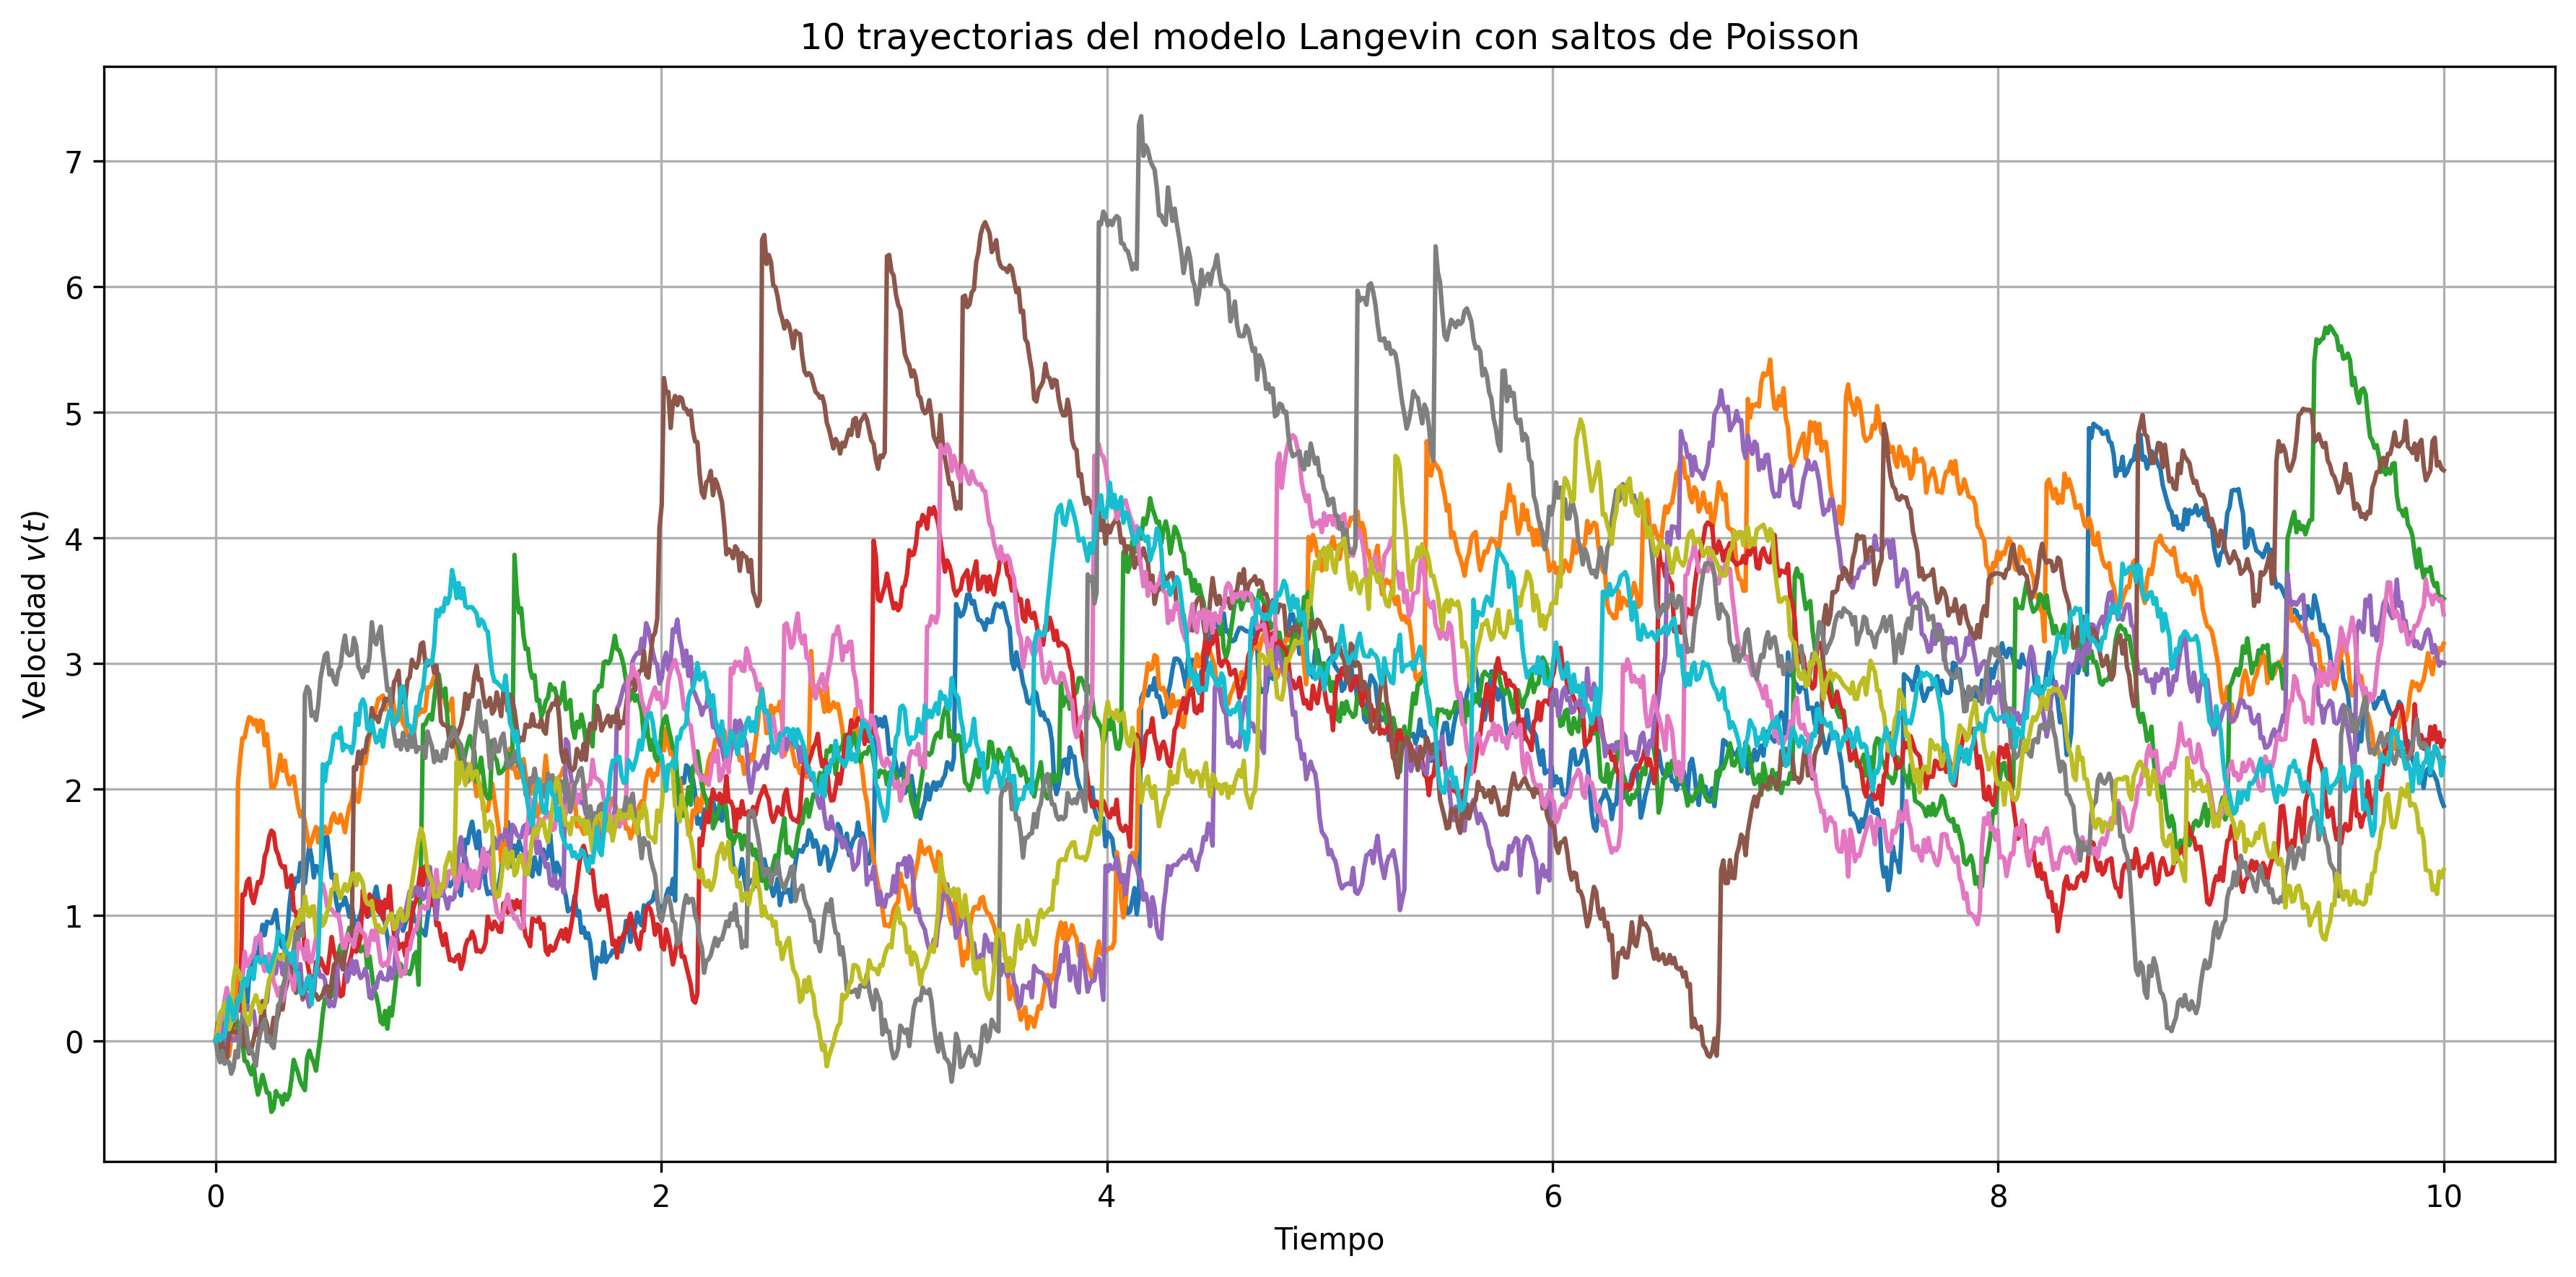
\includegraphics{chapters/presentacion_files/figure-pdf/cell-2-output-1.png}

}

\end{figure}

\begin{verbatim}
Matriz de transición de Markov basada en trayectorias simuladas:
          Micro  Minor  Moderate  Strong
Micro     0.922  0.078     0.000   0.000
Minor     0.022  0.945     0.032   0.001
Moderate  0.001  0.057     0.923   0.019
Strong    0.001  0.000     0.060   0.938
\end{verbatim}

\begin{figure}[H]

{\centering 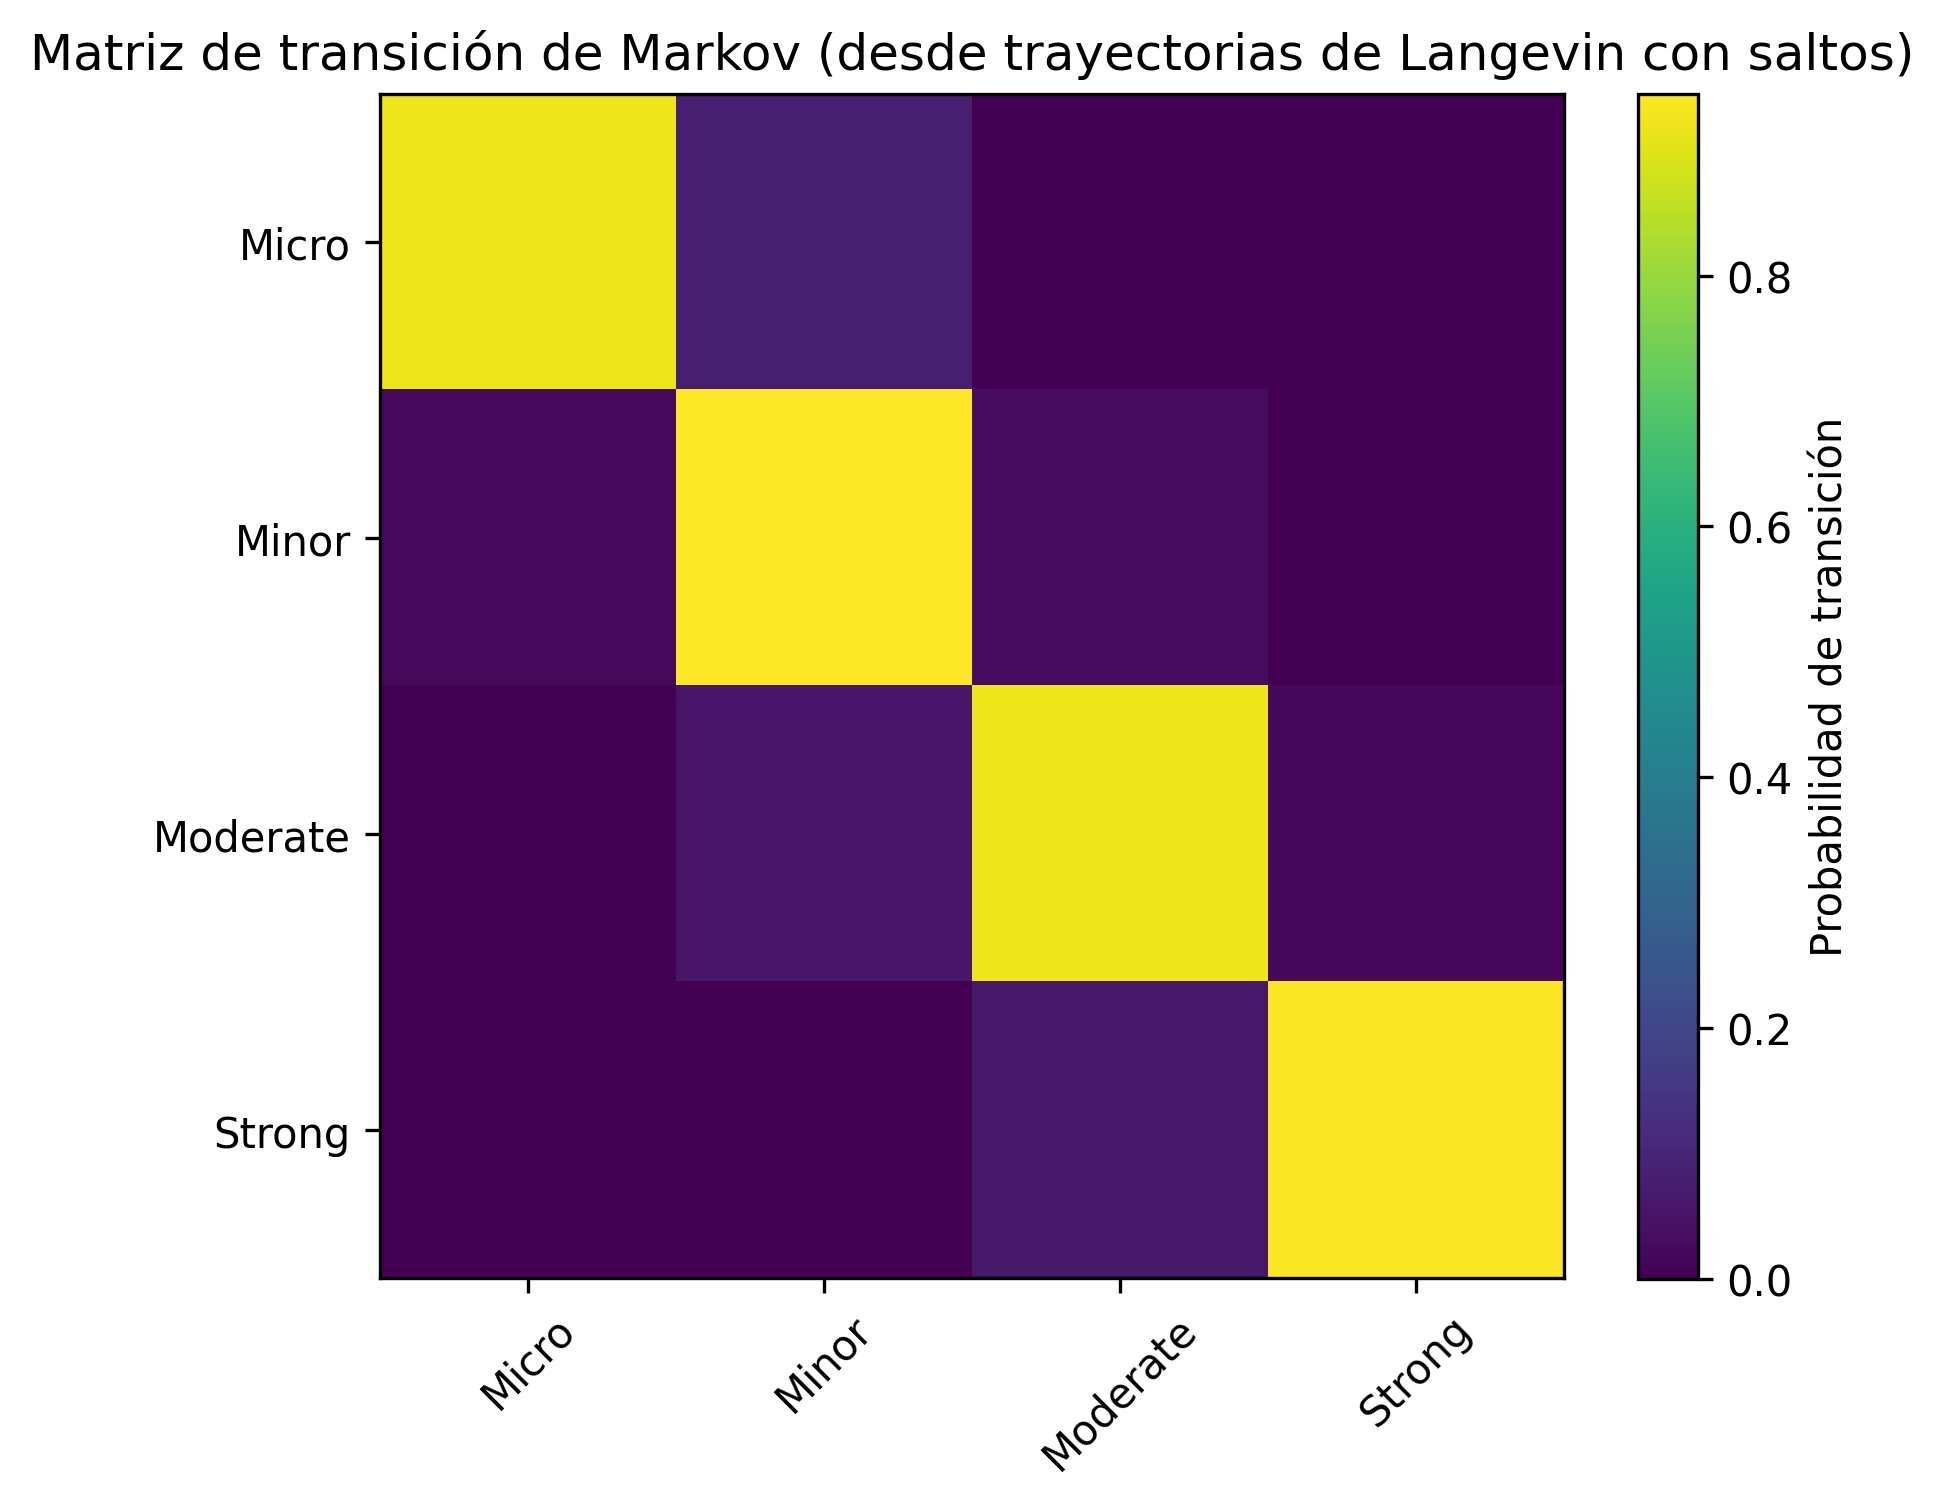
\includegraphics{chapters/presentacion_files/figure-pdf/cell-2-output-3.png}

}

\end{figure}

\bookmarksetup{startatroot}

\hypertarget{existencia-y-unicidad-fuerte}{%
\chapter{Existencia y unicidad
fuerte}\label{existencia-y-unicidad-fuerte}}

\begin{theorem}[]\protect\hypertarget{thm-varmues}{}\label{thm-varmues}

Sea \((\Omega, \mathcal{F}, (\mathcal{F}_t)_{t \geq 0}, \mathbb{P})\) un
espacio de probabilidad filtrado que satisface las hipótesis usuales.
Consideremos la \textbf{ecuación diferencial estocástica modificada}
(sin saltos grandes):

\begin{equation}\protect\hypertarget{eq-sde}{}{
\begin{aligned}
dZ(t) ={}& b(Z(t-)) \, dt \\
         &+ \sigma(Z(t-)) \, dB(t) \\
         &+ \int_{|x| < c} F(Z(t-), x) \, \widetilde{N}(dt, dx), \qquad t \geq 0,
\end{aligned}
}\label{eq-sde}\end{equation}

con condición inicial \(Z(0) = Z_0\), donde \(B(t)\) es un movimiento
browniano estándar unidimensional (\(r=1\)); \(N(dt, dx)\) es una medida
aleatoria de Poisson definida en
\(\mathbb{R}_+ \times (\mathbb{R} \setminus \{0\})\) con medida de
intensidad \(\nu(dx)\);
\(\widetilde{N}(dt, dx) = N(dt, dx) - \nu(dx)\,dt\) denota la
correspondiente medida compensada; \(c \in (0, \infty]\) es un umbral
fijo que separa los saltos pequeños de los grandes; y \(Z_0\) es una
variable aleatoria \(\mathcal{F}_0\)-medible, independiente del ruido
estocástico.

Supongamos que los coeficientes \(b: \mathbb{R} \to \mathbb{R}\),
\(\sigma: \mathbb{R} \to \mathbb{R}\) y
\(F: \mathbb{R} \times \mathbb{R} \to \mathbb{R}\) son funciones
\textbf{medibles} que satisfacen las siguientes condiciones:

\hypertarget{c1-condiciuxf3n-de-lipschitz}{%
\subsubsection*{\texorpdfstring{\textbf{(C1) Condición de
Lipschitz:}}{(C1) Condición de Lipschitz:}}\label{c1-condiciuxf3n-de-lipschitz}}
\addcontentsline{toc}{subsubsection}{\textbf{(C1) Condición de
Lipschitz:}}

Existe una constante \(K_1 > 0\) tal que, para todo
\(y_1, y_2 \in \mathbb{R}\),

\begin{equation}\protect\hypertarget{eq-lipschitz}{}{
\begin{aligned}
|b(y_1) - b(y_2)|^2 & + |\sigma(y_1) - \sigma(y_2)|^2\\ 
& + \int_{|x| < c} |F(y_1, x) - F(y_2, x)|^2 \, \nu(dx) \\
&\leq K_1 |y_1 - y_2|^2.
\end{aligned}
}\label{eq-lipschitz}\end{equation}

\hypertarget{c2-condiciuxf3n-de-crecimiento-lineal}{%
\subsubsection*{\texorpdfstring{\textbf{(C2) Condición de crecimiento
lineal:}}{(C2) Condición de crecimiento lineal:}}\label{c2-condiciuxf3n-de-crecimiento-lineal}}
\addcontentsline{toc}{subsubsection}{\textbf{(C2) Condición de
crecimiento lineal:}}

Existe una constante \(K_2 > 0\) tal que, para todo
\(y \in \mathbb{R}\),

\begin{equation}\protect\hypertarget{eq-3}{}{
|b(y)|^2 + |\sigma(y)|^2 + \int_{|x| < c} |F(y, x)|^2 \, \nu(dx)
\leq K_2 \bigl(1 + |y|^2 \bigr).
}\label{eq-3}\end{equation}

Bajo las hipótesis anteriores, existe una \textbf{única solución fuerte}
\(Z = (Z(t))_{t \geq 0}\) de la ecuación (Ecuación~\ref{eq-sde}) tal
que:

\begin{enumerate}
\def\labelenumi{\arabic{enumi}.}
\tightlist
\item
  \(Z\) es un \textbf{proceso adaptado y cádlág} (continuo por la
  derecha con límites por la izquierda),
\item
  La solución es única \textbf{casi seguramente,} esto es, si \((Z')\)
  es otra solución, entonces\\
  \begin{equation}\protect\hypertarget{eq-4}{}{
  \mathbb{P}\bigl(Z(t) = Z'(t) \text{ para todo } t \geq 0\bigr) = 1.
  }\label{eq-4}\end{equation}
\end{enumerate}

\end{theorem}

\begin{proof}

Queremos ver la existencia de una solución \(Z=(Z(t))_{t\geq 0}\) para
la ecuación (Ecuación~\ref{eq-sde}) con condición inicial \(Z(0)=Z_0\).
Bajo las hipótesis \textbf{(C1)} y \textbf{(C2)} para los coeficientes
\(b\), \(\sigma\) y \(F\). Ahora bien, la ecuación estocástica de
nuestro caso posee un movimiento browniano \(B\), es decir, ruido
estocástico y una medida de Poisson compensada, dada por
\(\widetilde{N}\), para esto utilizaremos la iteración de Picard
construyendo una sucesión de procesos estocásticos a partir de la
condición inicial. Definiendo la suceción de la siguiente forma:

\[
    Z_0(t) :=Z_0, \, \, \forall t\geq 0.
\]

Para \(n\geq 1\)

\[
    \begin{aligned}
        Z_{n+1}(t) := Z_0 & +\int _0^t b(Z_n(s-))ds+\int_0^t \sigma(Z(s-))dB(s)\\ 
        & + \int_0^t \int _{|x|<c} F(Z_n(s-),x)\widetilde{N}(ds,dx).
    \end{aligned}
\]

Demostraremos por inducción que el proceso \(Z_n\) es un proceso
adaptado y con trayectorias Cádlág. Así, para \(n=0\) consideremos la
diferencia \(Z_1(t)-Z_0(t)\). Por la iteración de Picard tenemos:

\[
    \begin{aligned}
        Z_1(t) = Z_0(t) & + \int_0^t b(Z_0(s-))ds +\int_0^t\sigma(Z_0(s-))\\ 
        & +\int_0^t \int_{|x|<c} F(Z_0(s-),x)\widetilde{N}(ds,dx).
    \end{aligned}
\]

Dado que \(Z_0(t)=Z_0\) para todo \(t\geq 0\), entonces,

\[
    \begin{aligned}
        Z_1(t)-Z_0 = \int_0^t b(Z_0) ds & + \int_0^t \sigma(Z_0)dB(s)\\ 
        & + \int_0^t\int_{|x|<c} F(Z_0,x)\widetilde{N}(ds,dx). 
    \end{aligned}
\]

Considerando la desigualdad

\[
(a+b+c)^2\leq 3(a^2+b^2+c^2).
\]

Tomando valor absoulto y elevando al cuadrado la expreción anterior
tenemos que

\begin{equation}\protect\hypertarget{eq-4}{}{
    \begin{aligned}
|Z_1(t)-Z_0|^2
&= \Bigg|
      \int_0^t b(Z_0)\,ds
      + \int_0^t \sigma(Z_0)\,dB(s) \\
&\qquad\quad
      + \int_0^t\!\!\int_{|x|<c} F(Z_0,x)\,\widetilde{N}(ds,dx)
   \Bigg|^2 \\[0.3em]
&\le 3\Bigg(
      \left(\int_0^t b(Z_0)\,ds\right)^2
      + \left(\int_0^t \sigma(Z_0)\,dB(s)\right)^2 \\
&\qquad\quad
      + \left(\int_0^t\!\!\int_{|x|<c} F(Z_0,x)\,\widetilde{N}(ds,dx)\right)^2
   \Bigg).
\end{aligned}
}\label{eq-4}\end{equation}

Para controlar de manera uniforme en todo el intervalo \([0,t]\) tomamos
el supremo sobre todo el intervalo, además usando propiedades del
supremos podemos obtener

\[
\begin{aligned}
\sup\limits_{0\leq s\leq t}|Z_1(t)-Z_0|^2
&\leq \sup\limits_{0\leq s\leq t}\Bigg(3\Bigg(
      \left(\int_0^t b(Z_0)\,ds\right)^2
      + \left(\int_0^t \sigma(Z_0)\,dB(s)\right)^2 \\
&\qquad\quad
      + \left(\int_0^t\!\!\int_{|x|<c} F(Z_0,x)\,\widetilde{N}(ds,dx)\right)^2
   \Bigg)\Bigg)\\
& = 3\Bigg(\sup\limits_{0\leq s\leq t}\left(\int_0^t b(Z_0)\,ds\right)^2 + \sup\limits_{0\leq s\leq t} \left(\int_0^t \sigma(Z_0)\,dB(s)\right)^2 \\ 
&\qquad\quad 
    + \sup\limits_{0\leq s\leq t} \left(\int_0^t\!\!\int_{|x|<c} F(Z_0,x)\,\widetilde{N}(ds,dx)\right)^2\Bigg).
\end{aligned}
\]

Tomando valor esperado de ambos lado y usando la linealidad, tenemos que

\[
\begin{aligned}
\mathbb{E}\Bigg[\sup\limits_{0\leq s\leq t}|Z_1(t)-Z_0|^2\Bigg]
& \leq \mathbb{E}\Bigg[3\Bigg(\sup\limits_{0\leq s\leq t}\left(\int_0^t b(Z_0)\,ds\right)^2\\
&\qquad   
    + \sup\limits_{0\leq s\leq t} \left(\int_0^t \sigma(Z_0)\,dB(s)\right)^2 \\ 
&\qquad\quad
    + \sup\limits_{0\leq s\leq t} \left(\int_0^t\!\!\int_{|x|<c} F(Z_0,x)\,\widetilde{N}(ds,dx)\right)^2\Bigg)\Bigg]\\
& = 3\Bigg( \mathbb{E}\Bigg[\sup\limits_{0\leq s\leq t}\left(\int_0^t b(Z_0)\,ds\right)^2\Bigg]\\ 
&\qquad
    + \mathbb{E}\Bigg[\sup\limits_{0\leq s\leq t} \left(\int_0^t \sigma(Z_0)\,dB(s)\right)^2\Bigg]\\
&\qquad\quad
    +\mathbb{E}\Bigg[\sup\limits_{0\leq s\leq t} \left(\int_0^t\!\!\int_{|x|<c} F(Z_0,x)\,\widetilde{N}(ds,dx)\right)^2\Bigg]\Bigg)
\end{aligned}
\]

Trabajaremos término por termino; así notemos que la siguiente integral
es de Lebesgue

\[
    \int_0^s b(z_0)du = b(z_0) \int_0^s du = b(z_0)\cdot s
\]

\end{proof}

\bookmarksetup{startatroot}

\hypertarget{referencias}{%
\chapter{Referencias}\label{referencias}}



\end{document}
